\subsection{Replication}

\subsubsection{Close Replication: Testing prior findings}
\begin{figure}[p]  % 'p' puts it on its own page
    \centering
    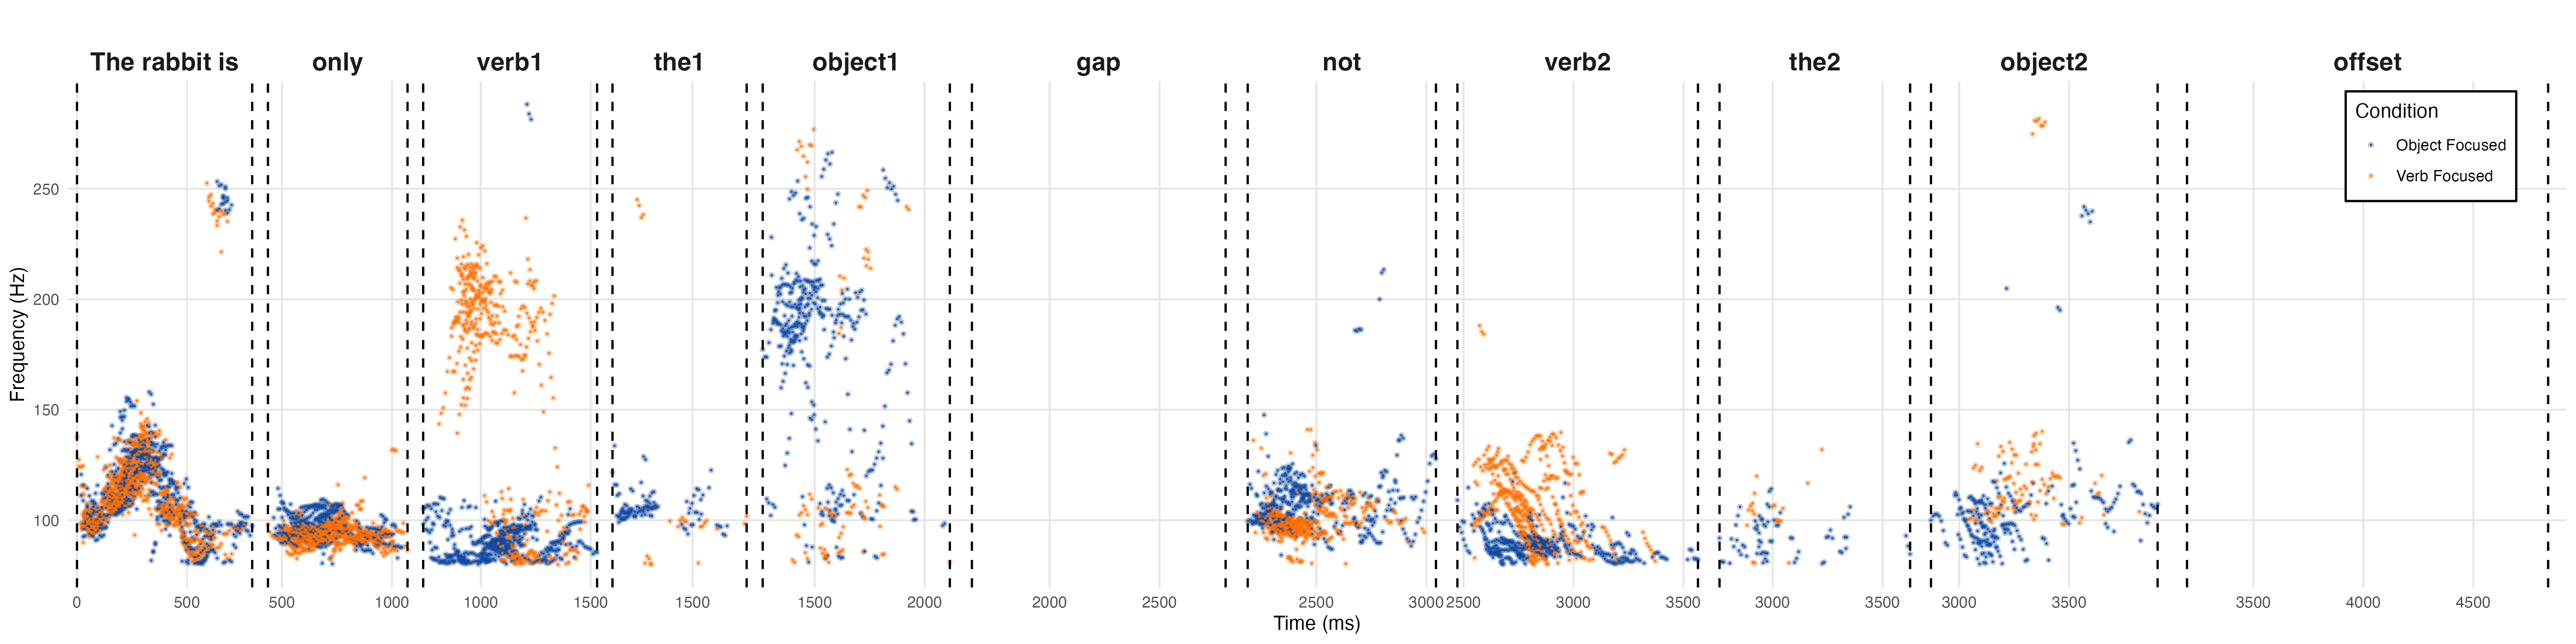
\includegraphics[width=\textwidth,height=\textheight,keepaspectratio]{viz/accoustic.png}
    \caption{things}
    \label{fig:acoustic}
\end{figure}



L1 

\subsubsection{Close Replication: Testing prior findings}
\begin{figure}[p]  % 'p' puts it on its own page
    \centering
    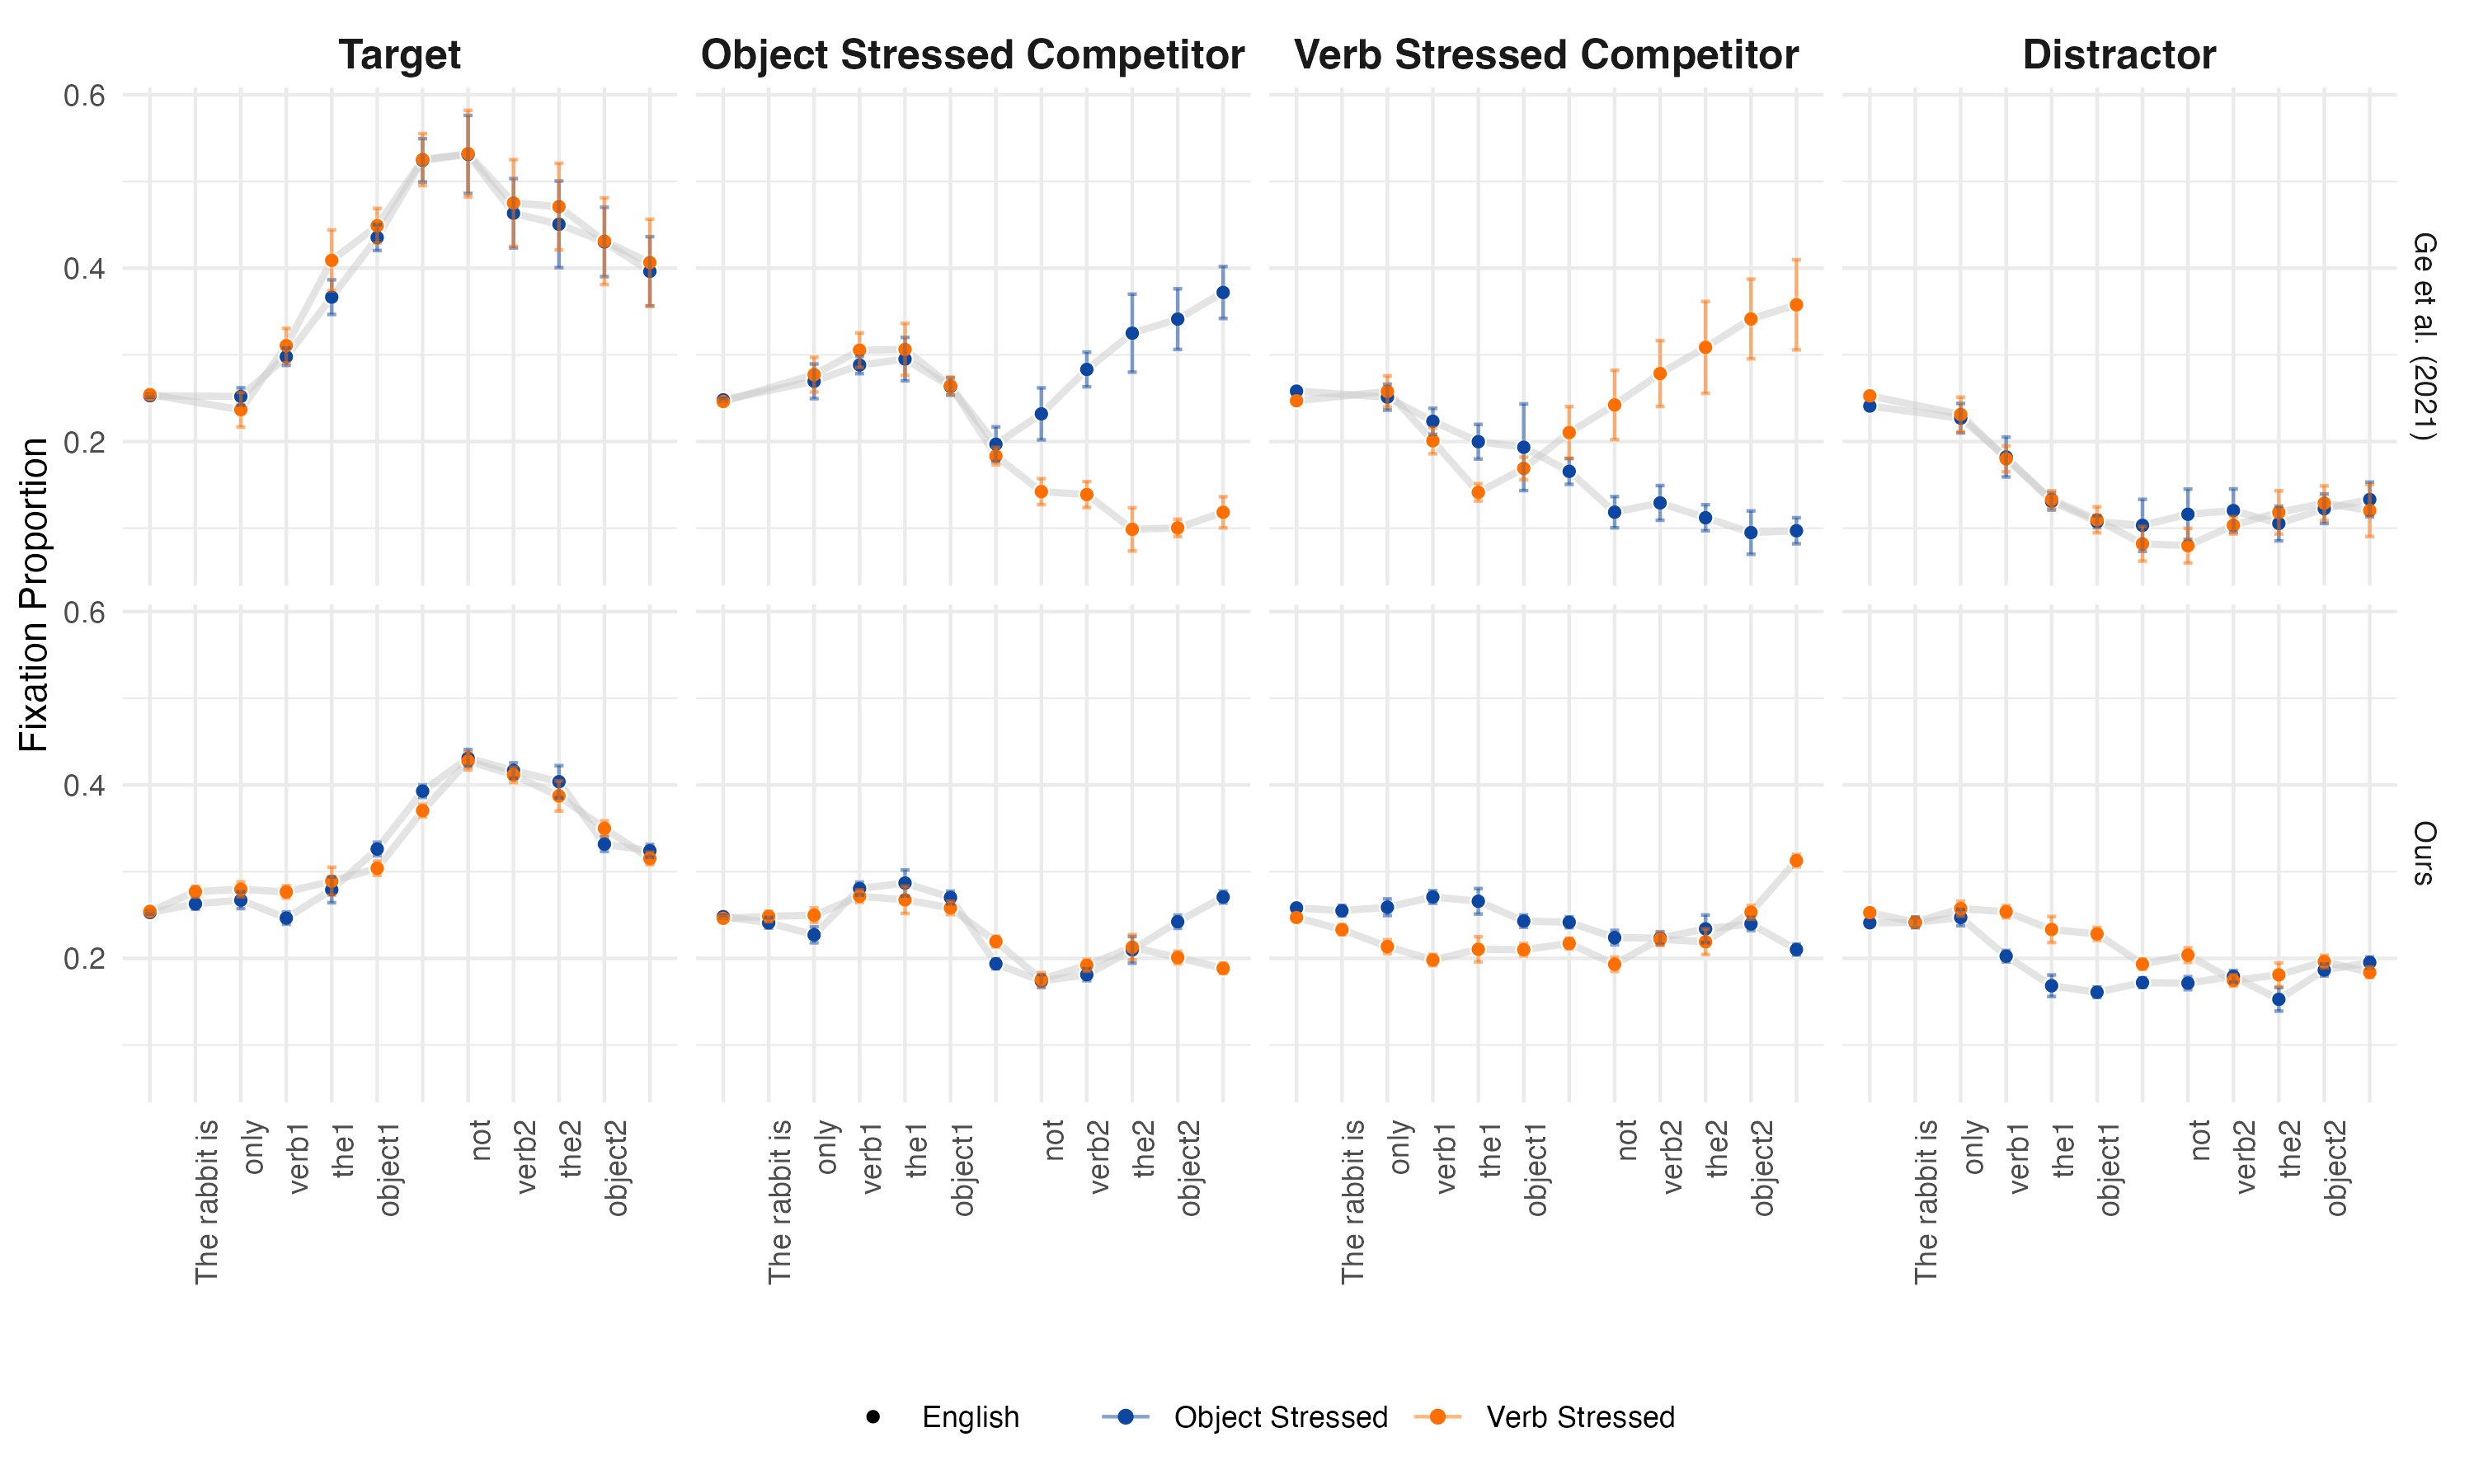
\includegraphics[width=\textwidth,height=\textheight,keepaspectratio]{viz/english_fix.png}
    \caption{things}
    \label{fig:english_fix}
\end{figure}



L2

\subsubsection{Close Replication: Testing prior findings}
\begin{figure}[p]  % 'p' puts it on its own page
    \centering
    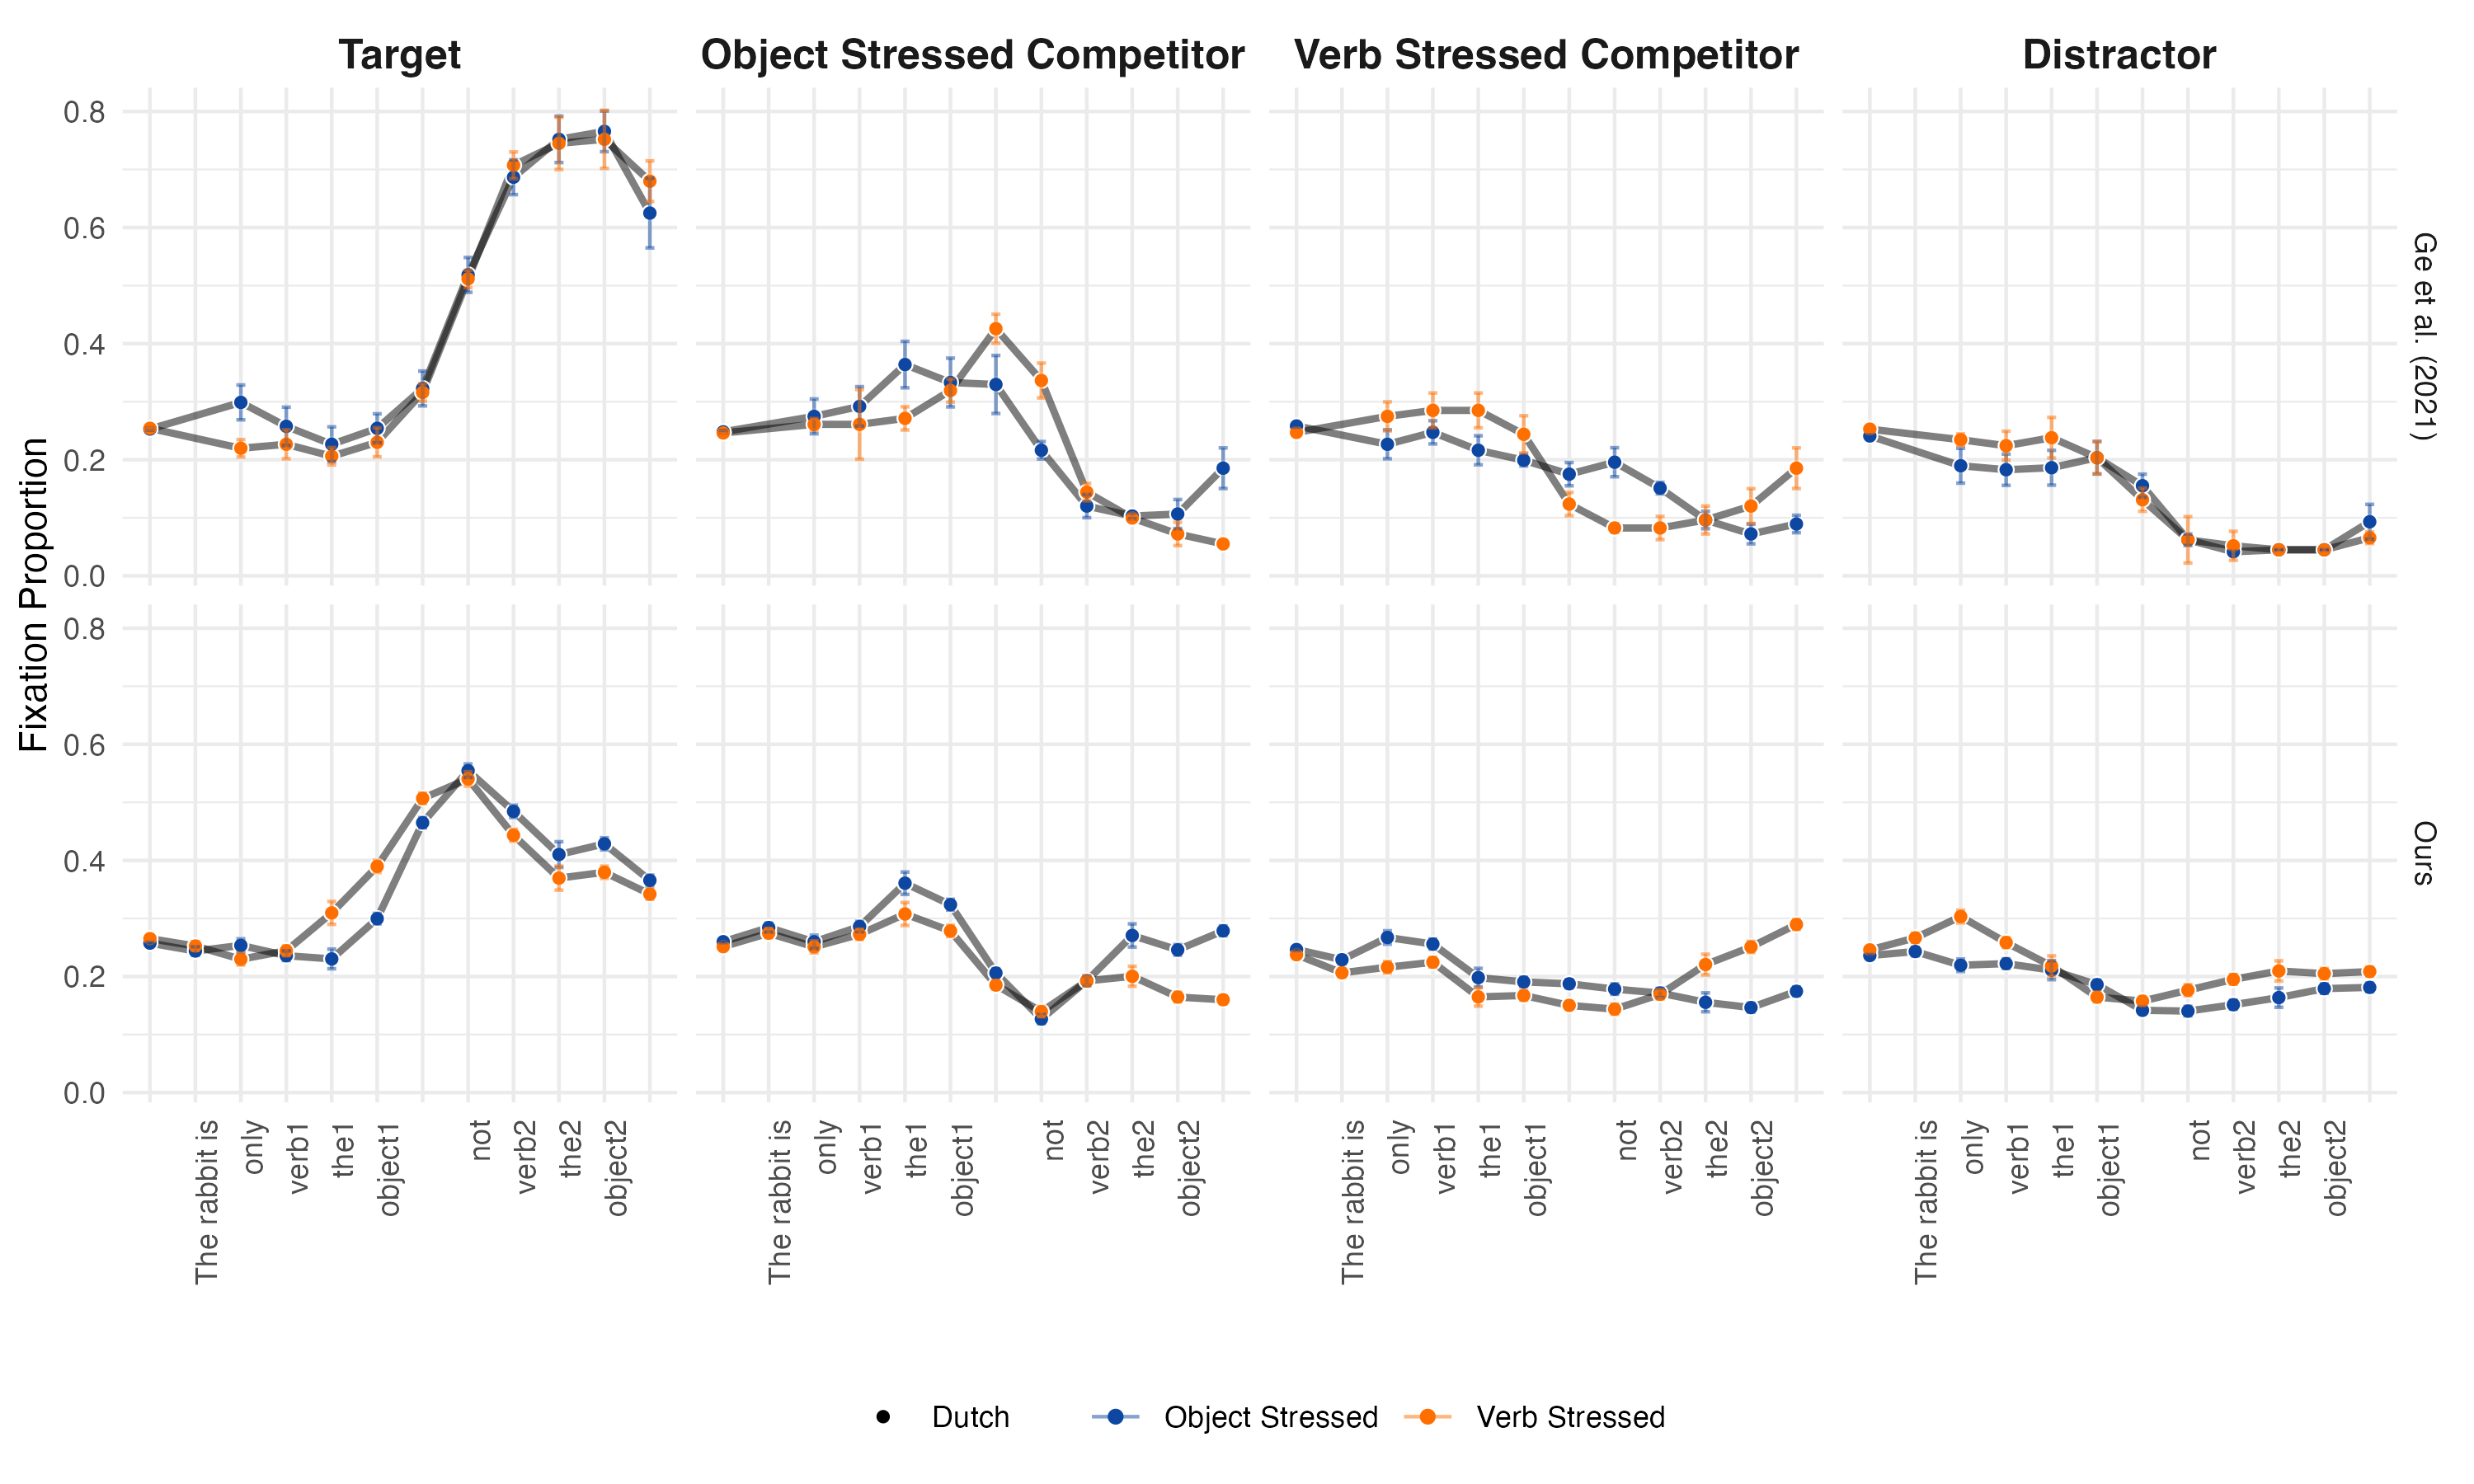
\includegraphics[width=\textwidth,height=\textheight,keepaspectratio]{viz/dutch_fix.png}
    \caption{things}
    \label{fig:dutch_fix}
\end{figure}

\subsubsection{Methodological refinement: A "focused" approach}

L1 

L2

\subsection{Extension}

Individual difference plot:
\clearpage
\begin{figure}[p]  % 'p' puts it on its own page
    \centering
    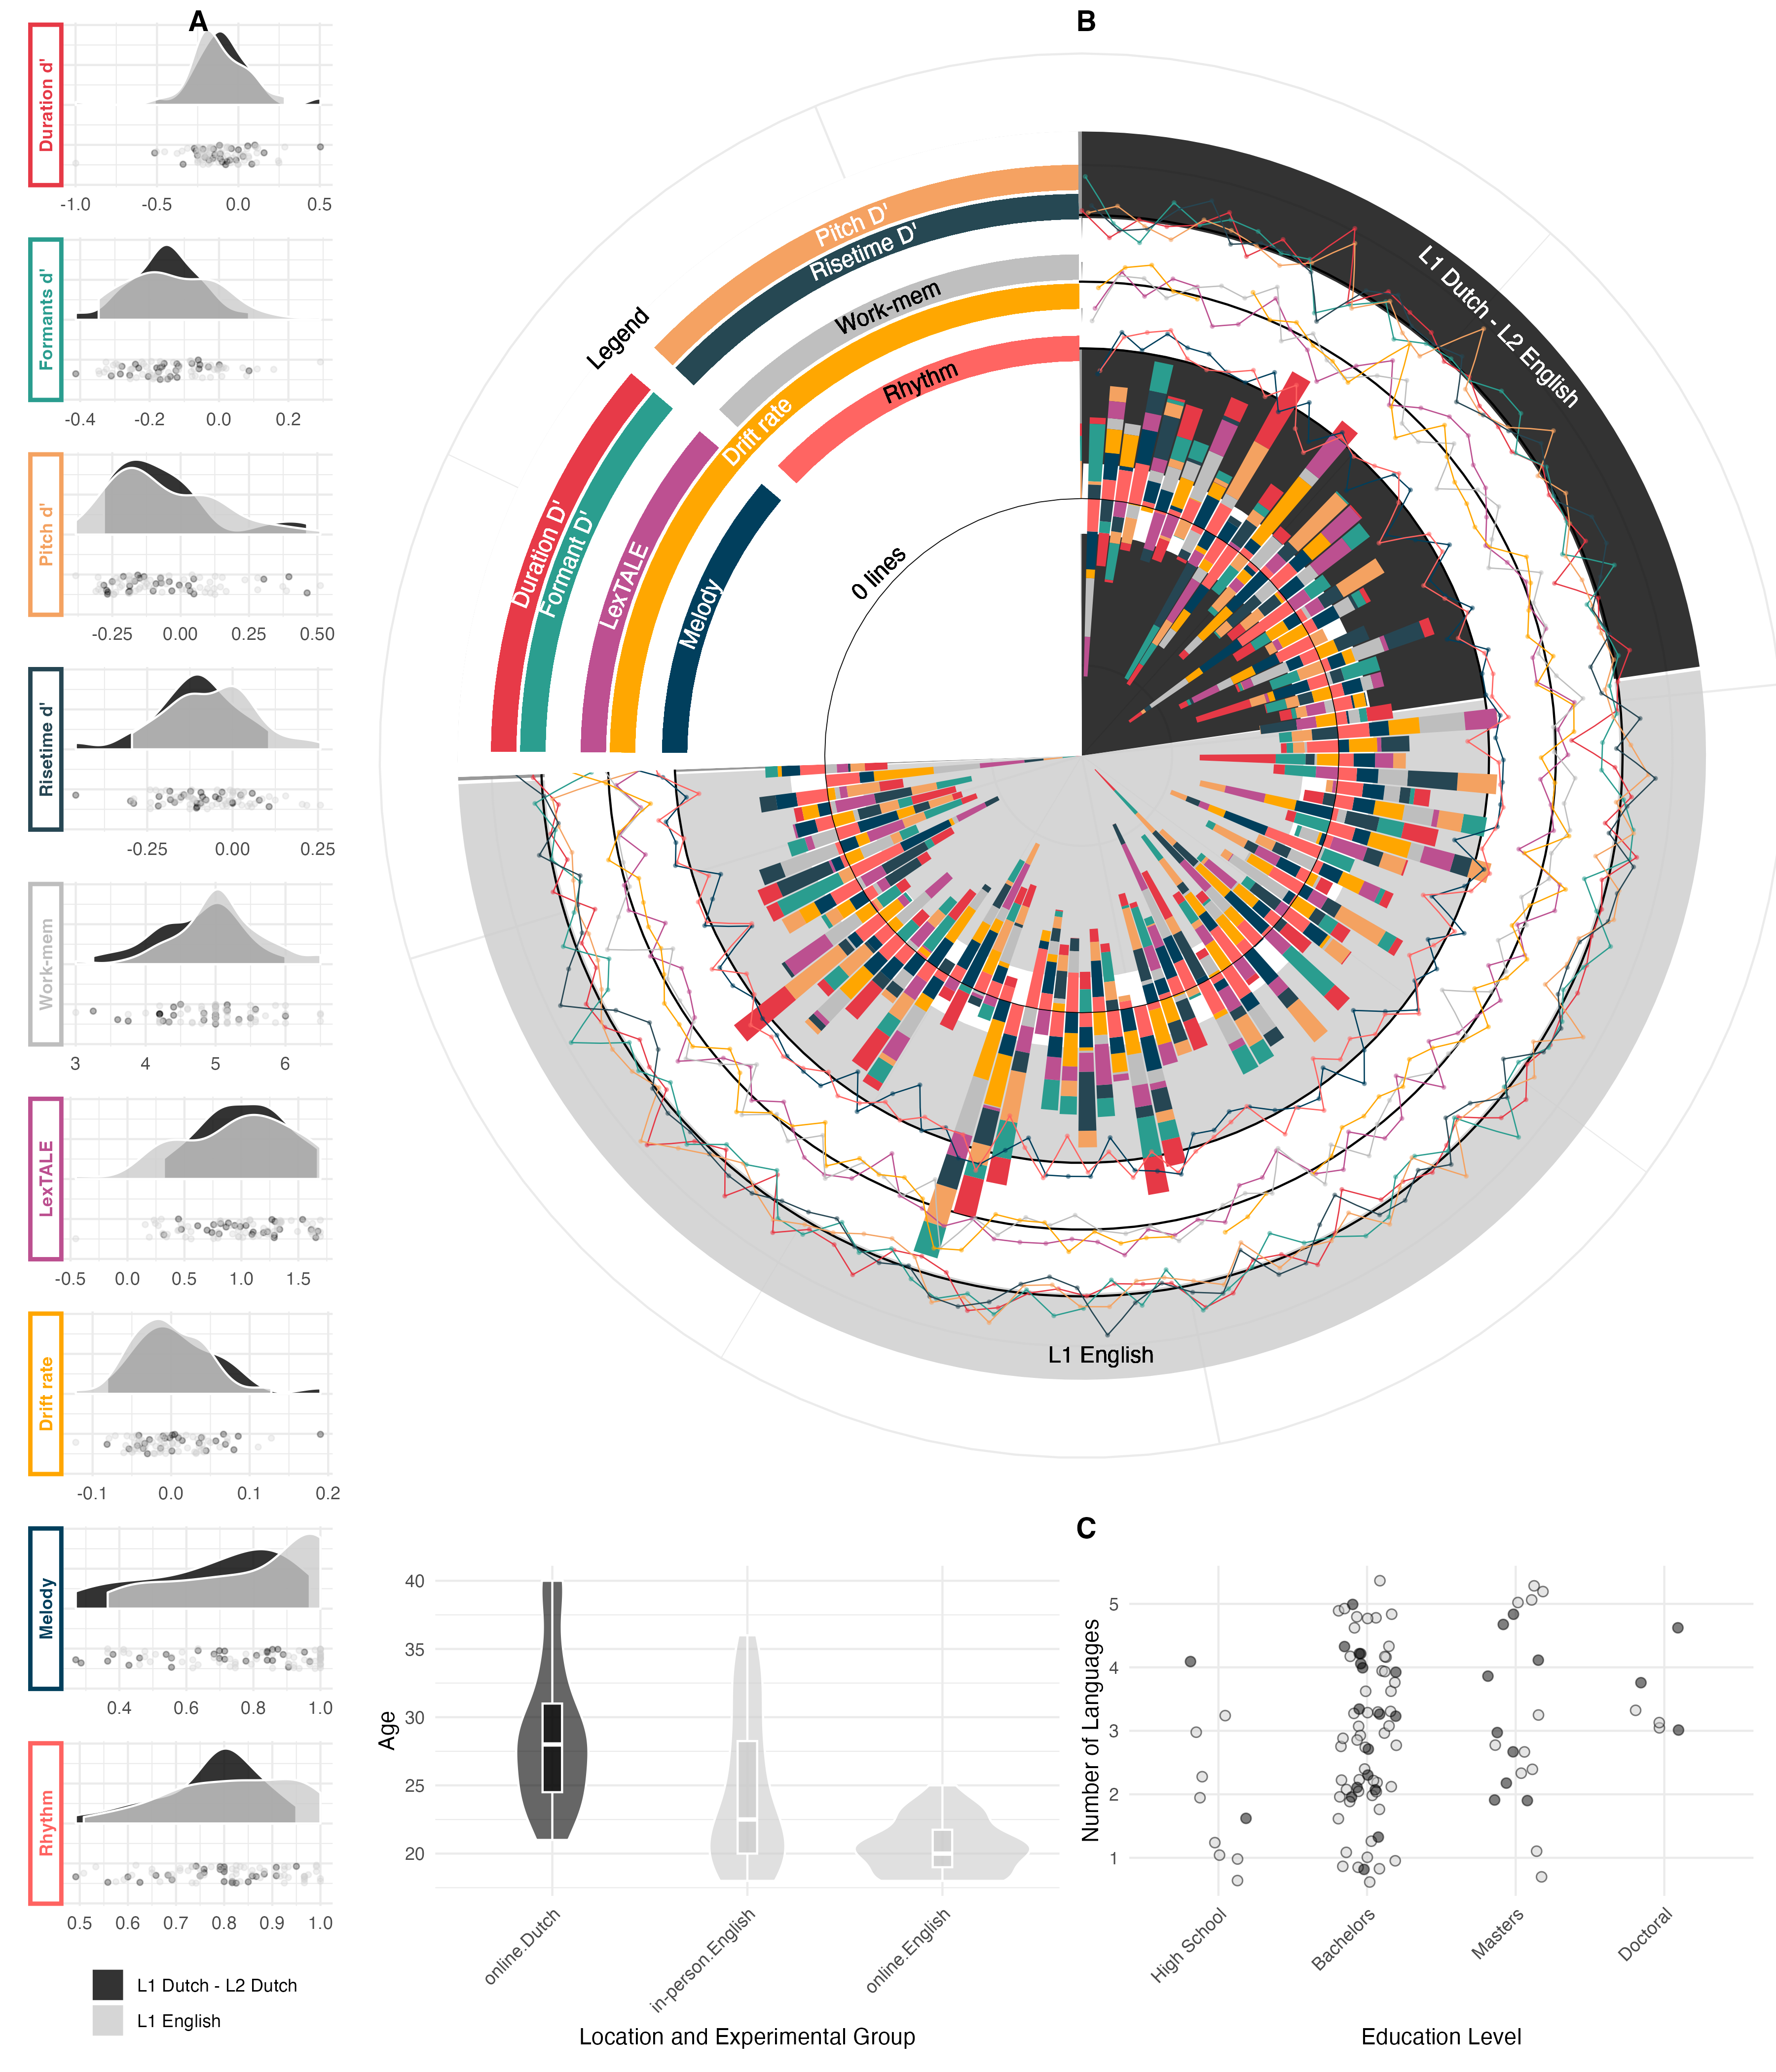
\includegraphics[width=\textwidth,height=\textheight,keepaspectratio]{viz/combined_plot_circle.png}
    \caption{describe what is going on here- A- tasks across the Dutch and English, B individual difference vectors for each participant, C background information on participants}
    \label{fig:combined_plot}
\end{figure}
\clearpage

L1 

L2


